\section{Einleitung}
Ähnlich wie der Lebensraum der Fische auf das Wasser begrenzt ist, so ist unser 
Lebensraum begrenzt auf das Universum.
Weiss ein Fisch, wie das Meer von unserem Blickpunkt aus aussieht?
Wahrscheinlich nicht, wieso sollte ihn das auch interessieren?
Da wir aber keine Fische sind, ist es nur natürlich sich zu fragen, wie das 
Universum von Aussen betrachtet, aussieht.
Um die Frage nach der Form des Universums beantworten zu können, werden wir uns 
im folgenden Kapitel mit dem kosmischen Mikrowellenhintergrund befassen.

\subsection{Der kosmische Mikrowellenhintergrund}
Glaubt man der Theorie des Big-Bang, (was wir im folgenden tun wollen) so waren 
der Druck und die Temperaturen in den ersten ca. 380'000 Jahren nach dem 
Big-Bang so, dass Atome nicht existieren konnten.
Die gesamte Masse bestand stattdessen aus ionisiertem Plasma, welches sehr 
effizient darin war, Strahlung zu zerstreuen (dieser Effekt ist unter 
Thomson-Streuung bekannt).
Dadurch ist es Forschern heute unmöglich, nachzuvollziehen, was in dieser Zeit 
passiert ist.
Das einzige was wir heute sehen, wenn wir weit genug in der Zeit zurückblicken,
ist eine Art Explosion (siehe Abbildung \ref{fig:radiation_scattering}).
Wir wissen nicht genau was darin passiert ist, doch wir wissen dass sie passiert ist.
\begin{figure}
	\centering
	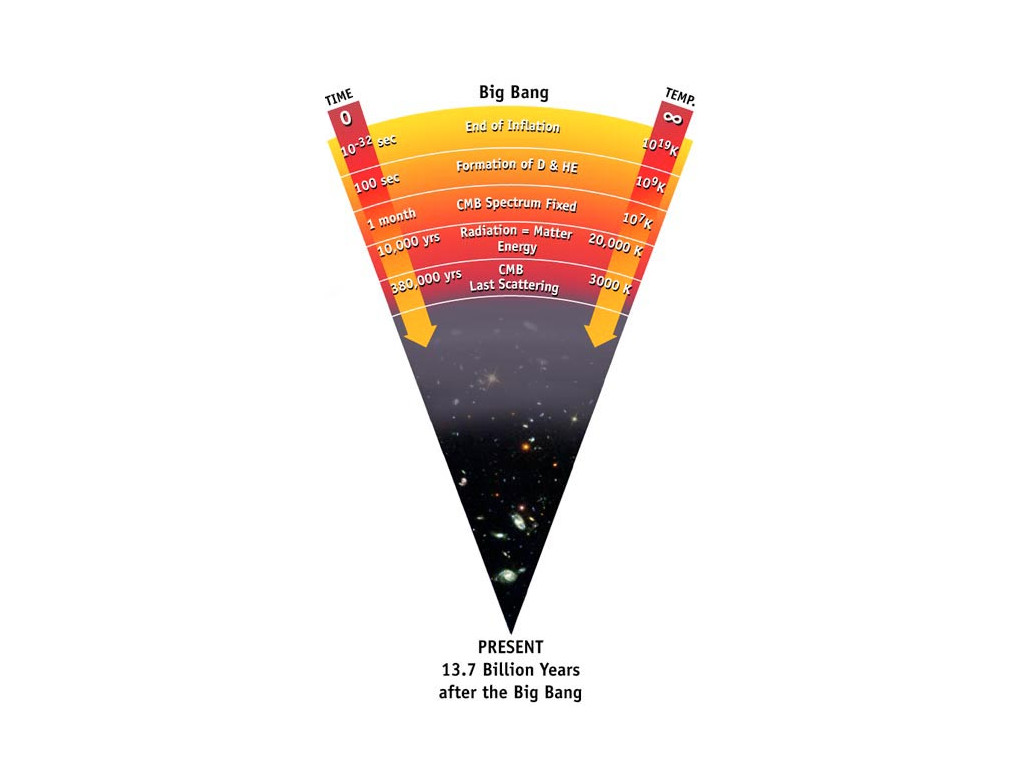
\includegraphics[width=\linewidth]{cmb/images/radiation_scattering.jpg}
	\caption{Sichtbarkeit des Universums im Zeitverlauf}
	\label{fig:radiation_scattering}
\end{figure}


Im Verlauf der nächsten 380'000 Jahre (relativ gesehen ein sehr kurzer Zeitraum) und der damit verbundenen Ausdehnung des 
Universums sanken Druck und damit die Temperatur im Universum stark, nämlich auf ungefähr 3700 
Kelvin.
Nun waren die Bedingungen erfüllt, dass sich Protonen und Elektronen zu 
Wasserstoffatomen verbinden konnten.
Die Zeit in der sich die ersten Atome bildeten, ist auch als Rekombination bekannt.


Nach dieser Rekombination gab es keine freien Elektronen mehr, wodurch die 
Photonen nicht mehr durch Thomson-Streuung abgelenkt wurden.
Den Photonen war es jetzt endlich möglich, der ``Explosion des Big-Bang'' zu 
entkommen und sich frei zu bewegen.
Die kosmische Mikrowellenhintergrundstrahlung ist eine Aufzeichnung der Photonen zum 
Zeitpunkt der Rekombination und verfügt über das thermische Spektrum einer Schwarzkörperstrahlung.

Abbildung \ref{fig:blackbody_spectrum} zeigt, dass Temperatur und Wellenlänge einer Schwarzkörperstrahlung proportional sind.
Aufgrund dieser Proportionalität lässt sich genau vorhersagen, welche Temperatur der kosmische Mikrowellenhintergrund zu welcher Zeit hatte.
\begin{figure}
	\centering
	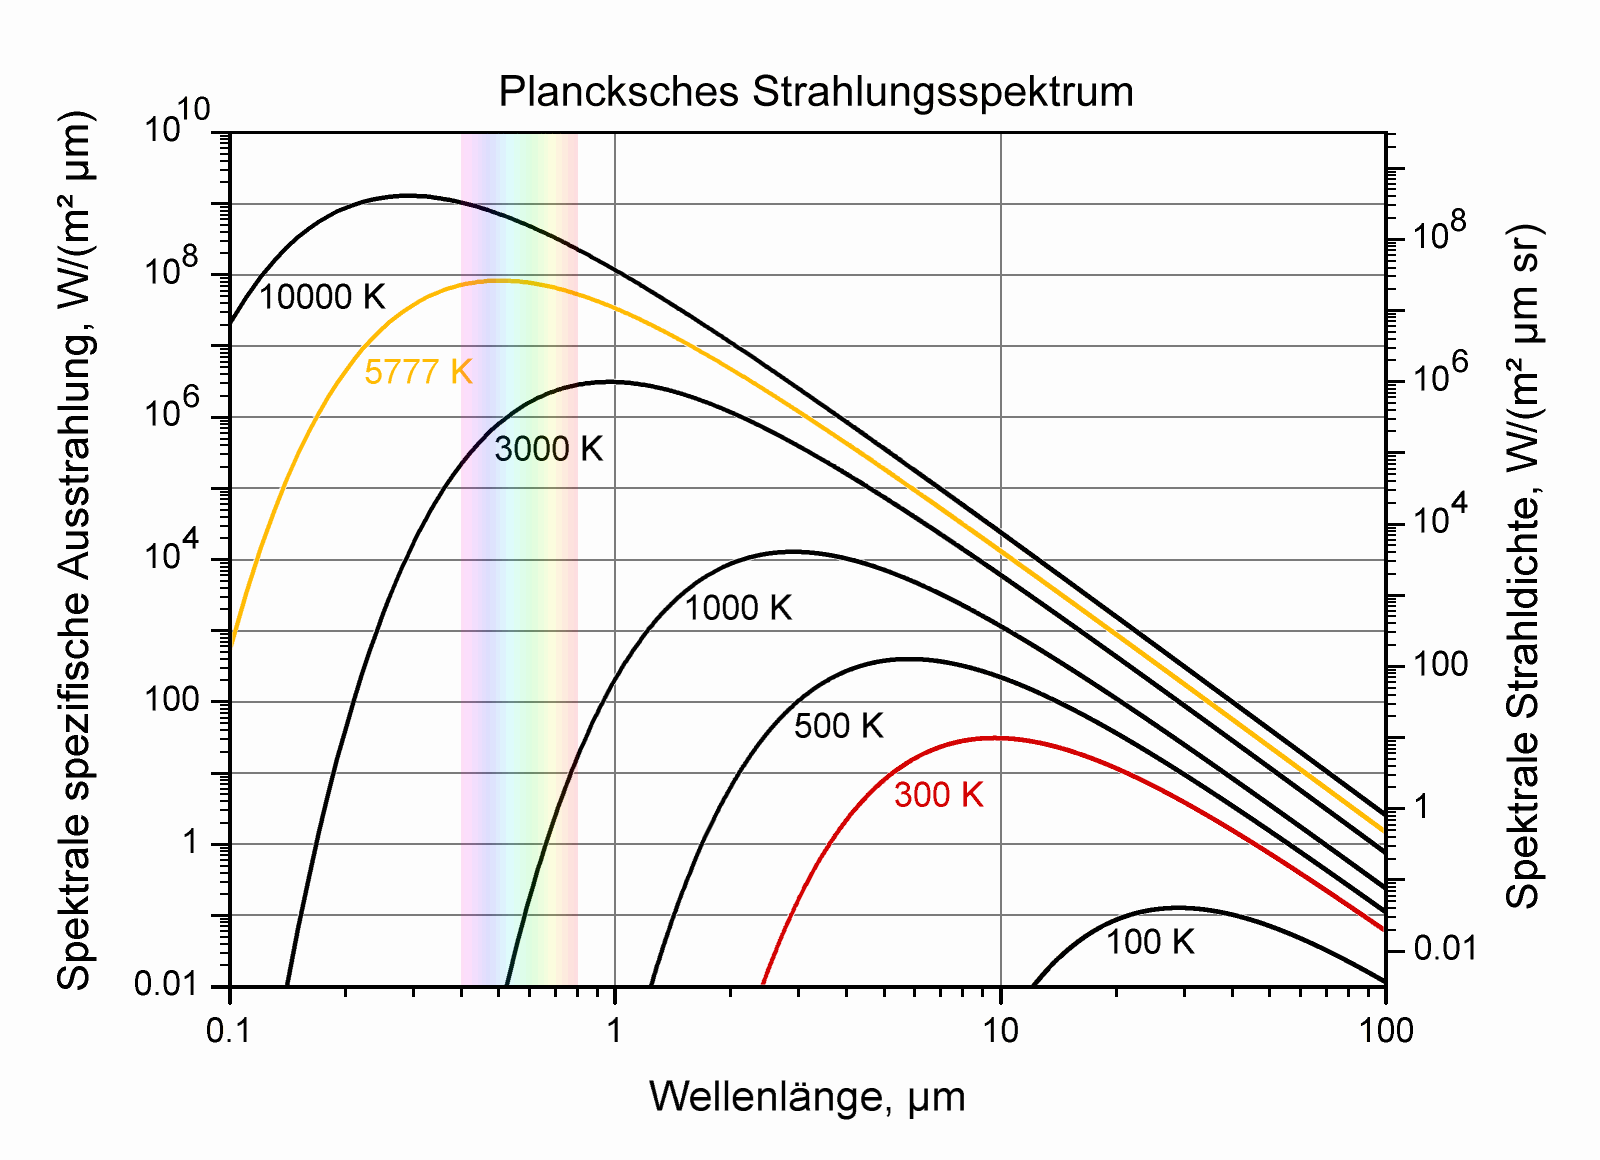
\includegraphics[width=\linewidth]{cmb/images/blackbody_spectrum.png}
	\caption{Plancksche Strahlungsspektren für verschiedene Temperaturen in doppeltlogarithmischer Auftragung}
	\label{fig:blackbody_spectrum}
\end{figure}
(Dieser Fakt ist essentiell für die spätere Entdeckung der Strahlung).
\ref{CMB_intro}

\section{Die Entdeckung des kosmischen Mikrowellenhintergrunds}
Nachdem bereits zahlreiche Forscher erfolglos nach dem kosmischen 
Mikrowellenhintergrund gesucht hatten, geschah die tatsächliche Entdeckung der 
Strahlung, wie so oft in der Wissenschaft, per Zufall.
Im Jahr 1964 arbeiteten Arno Penzias und Robert Woodrow Wilson an einer 
sogenannten ``Large Horn Antenna'' (siehe Abbildung \ref{fig:wilson_penzias}).
\begin{figure}
	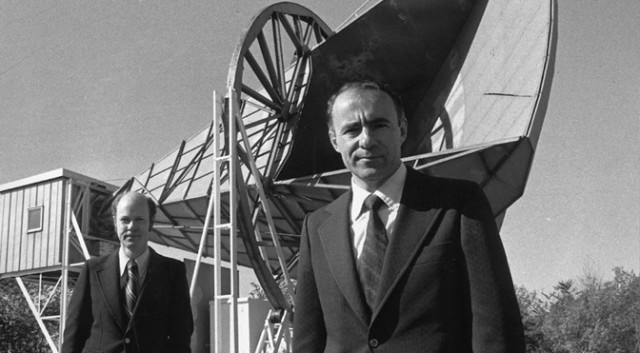
\includegraphics[width=\linewidth]{cmb/images/penzias-wilson-large-horn-antenna.jpg}
	\caption{Robert W. Wilson (links) und Arno A. Penzias vor ihrer Antenne}
	\label{fig:wilson_penzias}
\end{figure}
Dabei fanden sie ein Störsignal, welches unabhängig von der Ausrichtung der 
Antenne gleich war.
Dies ist der Grund weshalb der kosmische Mikrowellenhintergrund auf uns wirkt, als hätte er eine Kugelform
(die Strahlung wirkt von allen Richtungen gleichzeitig auf uns ein).
Deswegen haben die berühmten Bilder der Strahlung die Form einer plattgedrückten Kugel
(auch Mollweide-Projektion genannt).
Auch eine Reinigung der Antenne brachte keine Verbesserung, weshalb sie sich an 
andere Physiker wandten, welche bestätigten, dass es sich beim Störsignal um 
die erste Aufzeichnung der kosmischen Hintergrundstrahlung handelte.
Der Fund gilt als eine der wichtigsten Entdeckungen der Kosmologie und als 
Bestätigung der Urknalltheorie.
Deswegen wurde ihnen dafür 1978 der Nobelpreis für Physik verliehen.

In den Messungen von Wilson und Penzias wurde eine extreme Isotropie in der 
Strahlung festgestellt.
Dies stellte ein Problem dar, da dass heutige Universum sich nur gebildet haben 
konnte, wenn auch im Universum vor der Rekombination bereits Dichteschwankungen 
existiert haben.
Diese Schwankungen müssten auch in Temperaturunterschieden der kosmischen 
Hintergrundstrahlung erkennbar sein.
Fast 30 Jahre lang (1965-1992) blieb die Suche nach diesen Anisotropien 
erfolglos.
In dieser Zeit bemerkte man, dass die Temperaturschwankungen innerhalb der 
Strahlung extrem klein sein muss ($< 0.001\%$).
Die Erlösung brachte 1992 schliesslich der \ac{COBE} Satellit.
\ref{m_schoenitzer}